% Исходная версия шаблона --- 
% https://www.writelatex.com/coursera/latex/5.1

\documentclass[t]{beamer}  % [t], [c], или [b] --- вертикальное выравнивание на слайдах (верх, центр, низ)
%\documentclass[handout]{beamer} % Раздаточный материал (на слайдах всё сразу)
%\documentclass[aspectratio=169]{beamer} % Соотношение сторон

%\usetheme{Berkeley} % Тема оформления
%\usetheme{Bergen}
%\usetheme{Szeged}

%\usecolortheme{beaver} % Цветовая схема
%\useinnertheme{circles}
%\useinnertheme{rectangles}

\usetheme[protectframetitle]{m}

%%% Работа с русским языком
\usepackage{cmap}					% поиск в PDF
\usepackage{mathtext} 				% русские буквы в формулах
%\usepackage[T2A]{fontenc}			% кодировка
%\usepackage[utf8]{inputenc}			% кодировка исходного текста
\usepackage[english,russian]{babel}	% локализация и переносы

%% Beamer по-русски
\newtheorem{rtheorem}{Теорема}
\newtheorem{rproof}{Доказательство}
\newtheorem{rexample}{Пример}

%%% Дополнительная работа с математикой
\usepackage{amsmath,amsfonts,amssymb,amsthm,mathtools} % AMS
\usepackage{icomma} % "Умная" запятая: $0,2$ --- число, $0, 2$ --- перечисление

%% Номера формул
%\mathtoolsset{showonlyrefs=true} % Показывать номера только у тех формул, на которые есть \eqref{} в тексте.
%\usepackage{leqno} % Нумерация формул слева

%% Свои команды
\DeclareMathOperator{\sgn}{\mathop{sgn}}

%% Перенос знаков в формулах (по Львовскому)
\newcommand*{\hm}[1]{#1\nobreak\discretionary{}
{\hbox{$\mathsurround=0pt #1$}}{}}

%%% Работа с картинками
\usepackage{graphicx}  % Для вставки рисунков
\graphicspath{{images/}{images2/}}  % папки с картинками
\setlength\fboxsep{3pt} % Отступ рамки \fbox{} от рисунка
\setlength\fboxrule{1pt} % Толщина линий рамки \fbox{}
\usepackage{wrapfig} % Обтекание рисунков текстом

%%% Работа с таблицами
\usepackage{array,tabularx,tabulary,booktabs} % Дополнительная работа с таблицами
\usepackage{longtable}  % Длинные таблицы
\usepackage{multirow} % Слияние строк в таблице

%%% Программирование
\usepackage{etoolbox} % логические операторы

%%% Другие пакеты
\usepackage{lastpage} % Узнать, сколько всего страниц в документе.
\usepackage{soul} % Модификаторы начертания
\usepackage{csquotes} % Еще инструменты для ссылок
%\usepackage[style=authoryear,maxcitenames=2,backend=biber,sorting=nty]{biblatex}
\usepackage{multicol} % Несколько колонок

%%% Картинки
\usepackage{tikz} % Работа с графикой
\usepackage{pgfplots}
\usepackage{pgfplotstable}

%Библиография
\usepackage[backend=biber,bibencoding=utf8,sorting=nty,maxcitenames=4,style=gost-numeric, language=auto, babel=other]{biblatex}
\addbibresource{fuzzy_thesis.bib}

%DO NOT Insert frame with section title at every section start
% \AtBeginSection[]
% {
% }
\title{Поддержка принятия управленческих решений для развития урбанизированной
    территории на примере противодействия распространению наркомании в
    Санкт-Петербурге}
% \subtitle{Документы и презентации в \LaTeX}
\author{Великий Дмитрий Павлович \\ Научный руководитель: Захаров Юрий Никитич}
\date{\today}
\institute[ИТМО]{Университет ИТМО \\ Кафедра управления государственными
    информационными системами}
% \logo{
\includegraphics[height=2cm]{bw_rus.png}}

\begin{document}

\frame[plain]{\titlepage}	% Титульный слайд

% \section{Положения, выносимые на защиту}
\begin{frame}
    \frametitle{Положения, выносимые на защиту}%\protect\insertsection} 
	\begin{itemize}
        \item \alert{Модель} прогнозирования численности наркозависимых в
            Санкт-Петербурге;
        \item \alert{Компонент} Банка Данных ИС ИАО, предназначенный для анализа и
            прогнозирования динамики численности наркозависимых на территории
            Санкт-Петербурга.
	\end{itemize}
\end{frame}

% \section{Обзор антинаркотических политик}
\begin{frame}
    \frametitle{Обзор антинаркотических политик}%\protect\insertsection} 
	\begin{itemize}
        \item Снижение вреда;
        \item Снижение потребления.
	\end{itemize}
    Генеральная цель ---
    \begin{quote}
        существенное сокращение незаконного распространения и немедицинского 
        потребления наркотиков. \footfullcite{ru_nat_drug_strat}
    \end{quote}
\end{frame}
\begin{frame}
    \frametitle{Исходные данные}
    \textbf{Индикаторы воздействия}
    \begin{itemize}
    \item Социально-демографические и экономические;
    \item Медицинские;
    \item Криминальные.
    \end{itemize}
\end{frame}
% \section{Модель прогнозирования}
\plain{Модель прогнозирования}{}
% \subsection{Обучающий алгоритм}
\begin{frame}
    \frametitle{Обучающий алгоритм} 
    % \framesubtitle{\protect\insertsubsection} 
	\begin{block}{Нечеткая логика. \footfullcite{Wang1992}}
        \begin{enumerate}
            \item Разбиение областей определения;
            \item Генерация нечетких правил;
            \item Присвоение степеней правилам;
            \item Создание комбинированной нечеткой базы правил;
            \item Определение отображения входного пространства на выходное
                (дефаззификация).
        \end{enumerate}
	\end{block}

\end{frame}

\begin{frame}
    \frametitle{Методика анализа наркоситуации} 
	\begin{itemize}
        \item Учет коэффициента латентности;
        \item Анализ пороговых уровней;
        \item Перевод абсолютных значений численности наркозависимых в
            вероятность заболеваемости наркозависимостью.
	\end{itemize}
\end{frame}

\begin{frame}
    \frametitle{Компонент Банка данных ИС ИАО}
    \begin{figure}
        \centering
        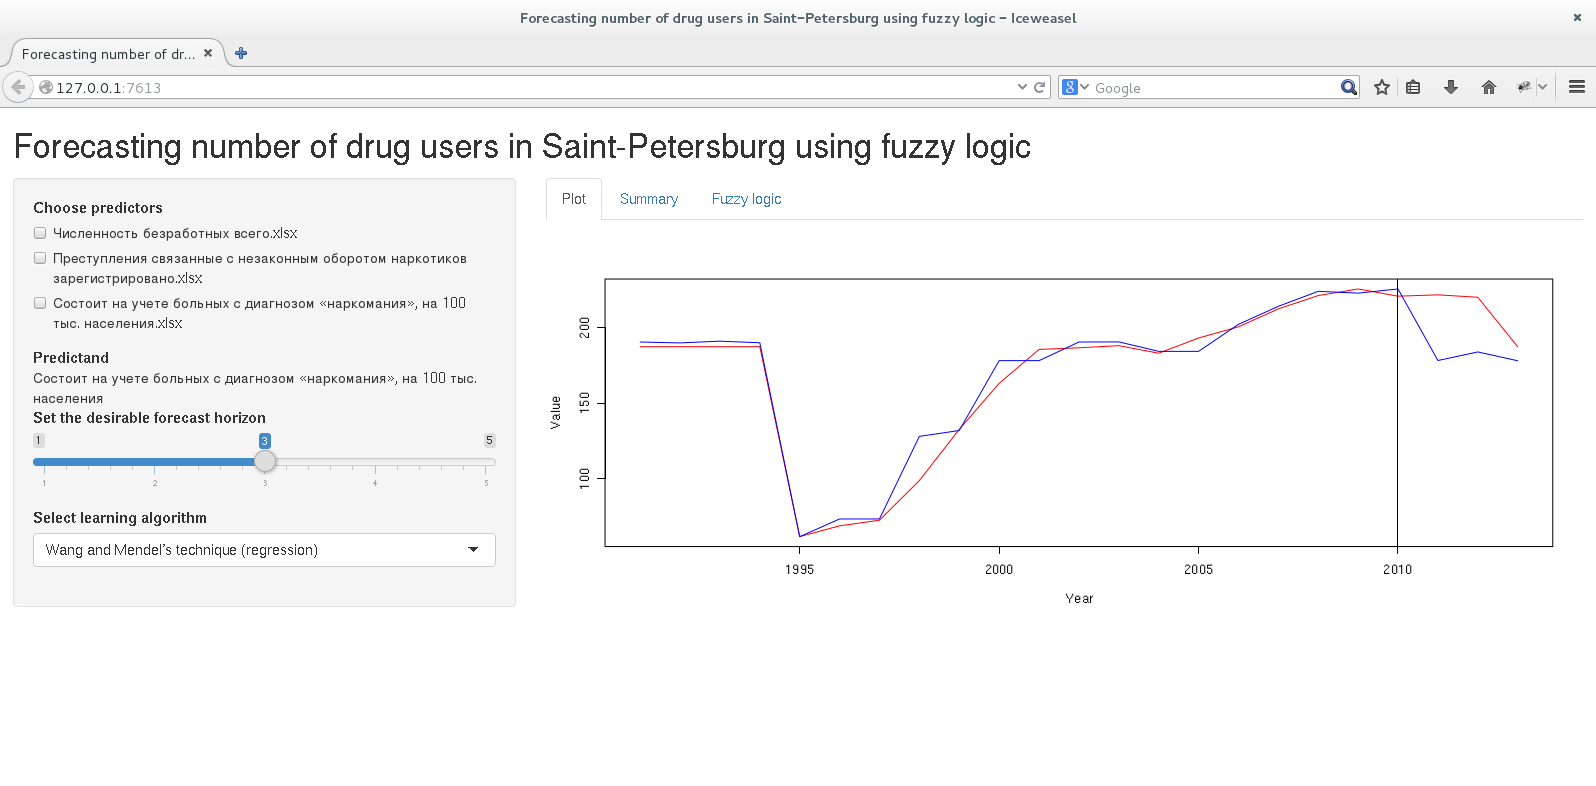
\includegraphics[width=\textwidth]{screenshot1.png}
    \end{figure}
    \url{http://tiny.cc/FuzzyForecast}
\end{frame}
\begin{frame}
    \frametitle{Компонент Банка данных ИС ИАО}
    \begin{figure}
        \centering
        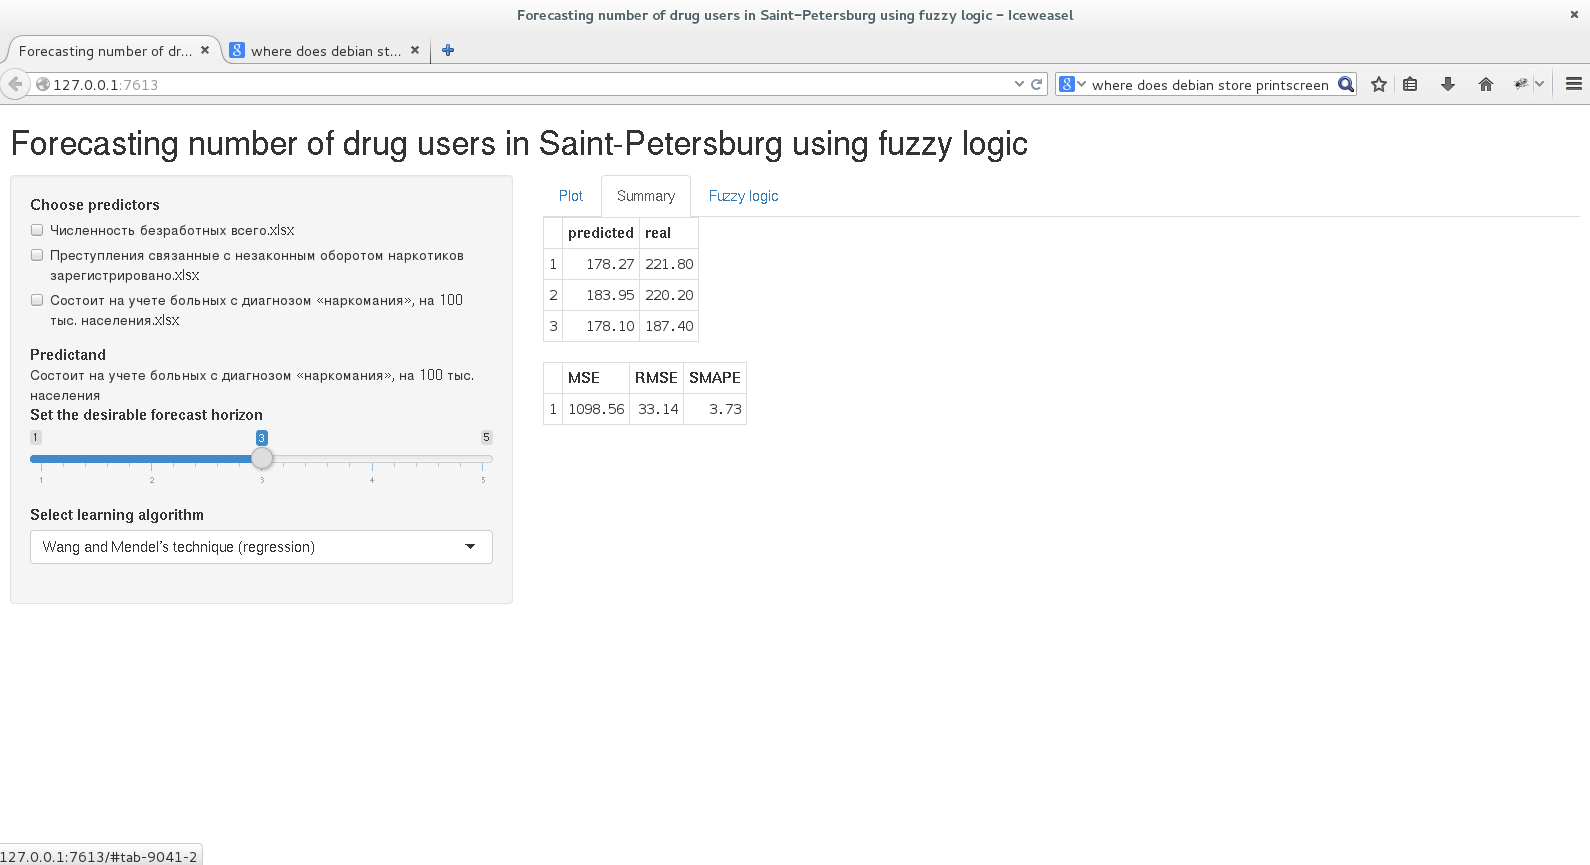
\includegraphics[width=\textwidth]{screenshot2.png}
    \end{figure}
\end{frame}
\begin{frame}
    \frametitle{Компонент Банка данных ИС ИАО}
    \begin{figure}
        \centering
        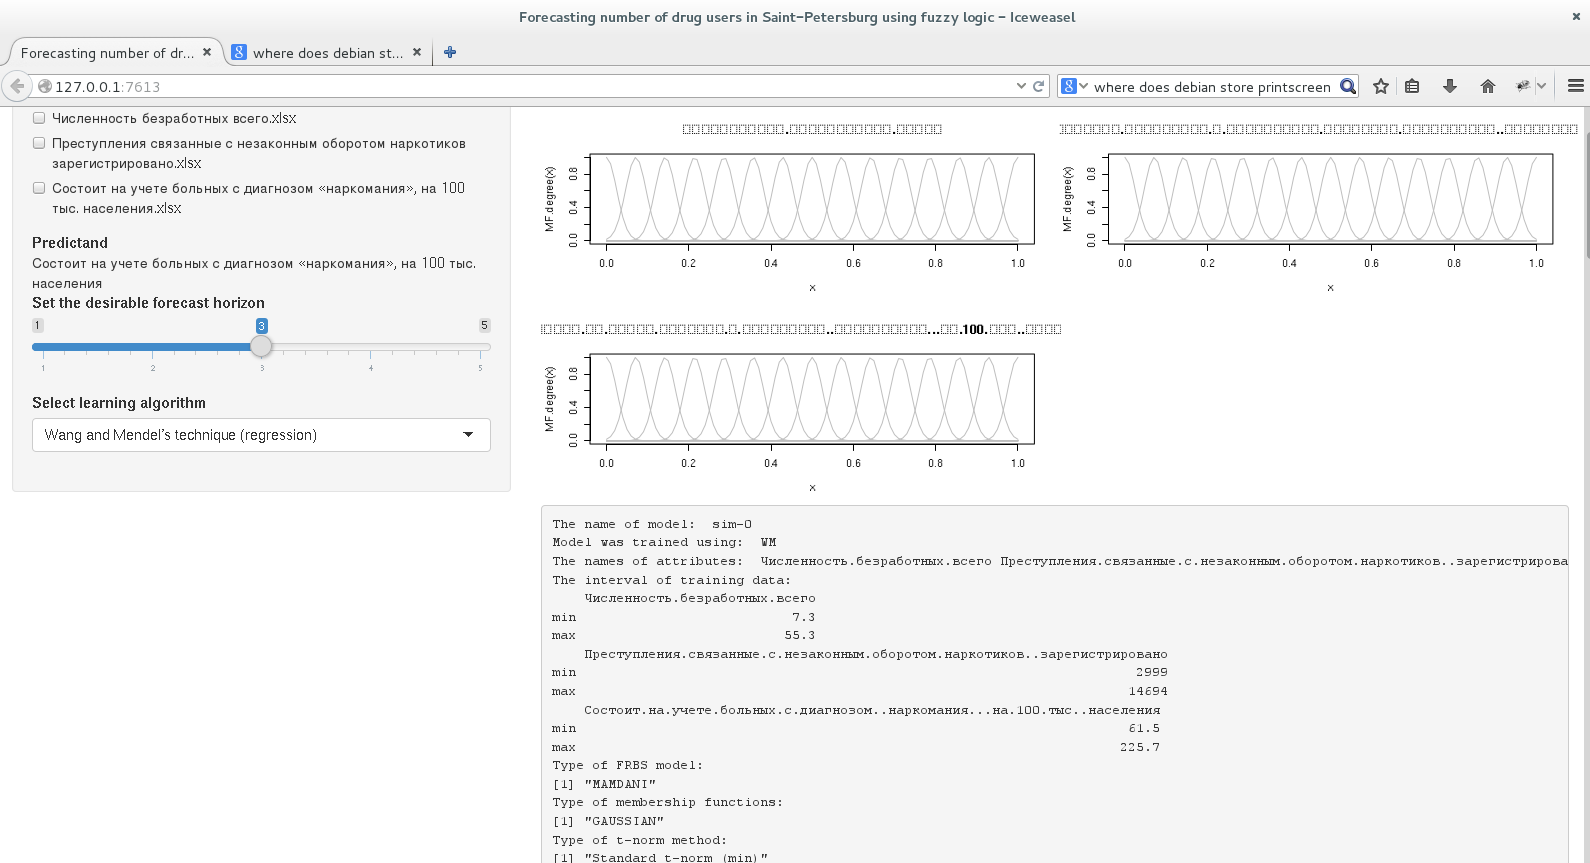
\includegraphics[width=\textwidth]{screenshot3.png}
    \end{figure}
\end{frame}
\begin{frame}
    \frametitle{Нечеткие правила}
    \textbf{IF} Численность безработных всего is \alert{v.1\_a.15} 
    
    \textbf{AND} Преступления, связанные с незаконным оборотом наркотиков зарегистрировано is
    \alert{v.2\_a.1} 

    \textbf{THEN} Состоит на учете больных с диагнозом наркомания на 100 тыс населения is
    \alert{c.1}
\end{frame}
\begin{frame}
    \frametitle{Преимущества метода}
    \begin{itemize}
        \item Моделирование связей между показателями;
        \item Возможность учета суждений экспертов;
        \item Адаптируемость под исходные данные.
    \end{itemize}

\end{frame}
\begin{frame}
    \frametitle{Направления развития}
    \begin{itemize}
        \item Сравнение результатов модели с аналогами из Банка моделей;
        \item Повышение юзабилити модели для ППР органов гос. власти.
    \end{itemize}
\end{frame}
\begin{frame}
    \frametitle{Спасибо за внимание!}
    \begin{block}{Великий Дмитрий Павлович}
        Поддержка принятия управленческих решений для развития урбанизированной
        территории на примере противодействия распространению наркомании в
        Санкт-Петербурге
    \end{block}
\end{frame}

\end{document}
